\section{Hiện thực hệ thống}
\subsection{Hiện thực phần cứng}
\begin{figure}[H]
    \centering
    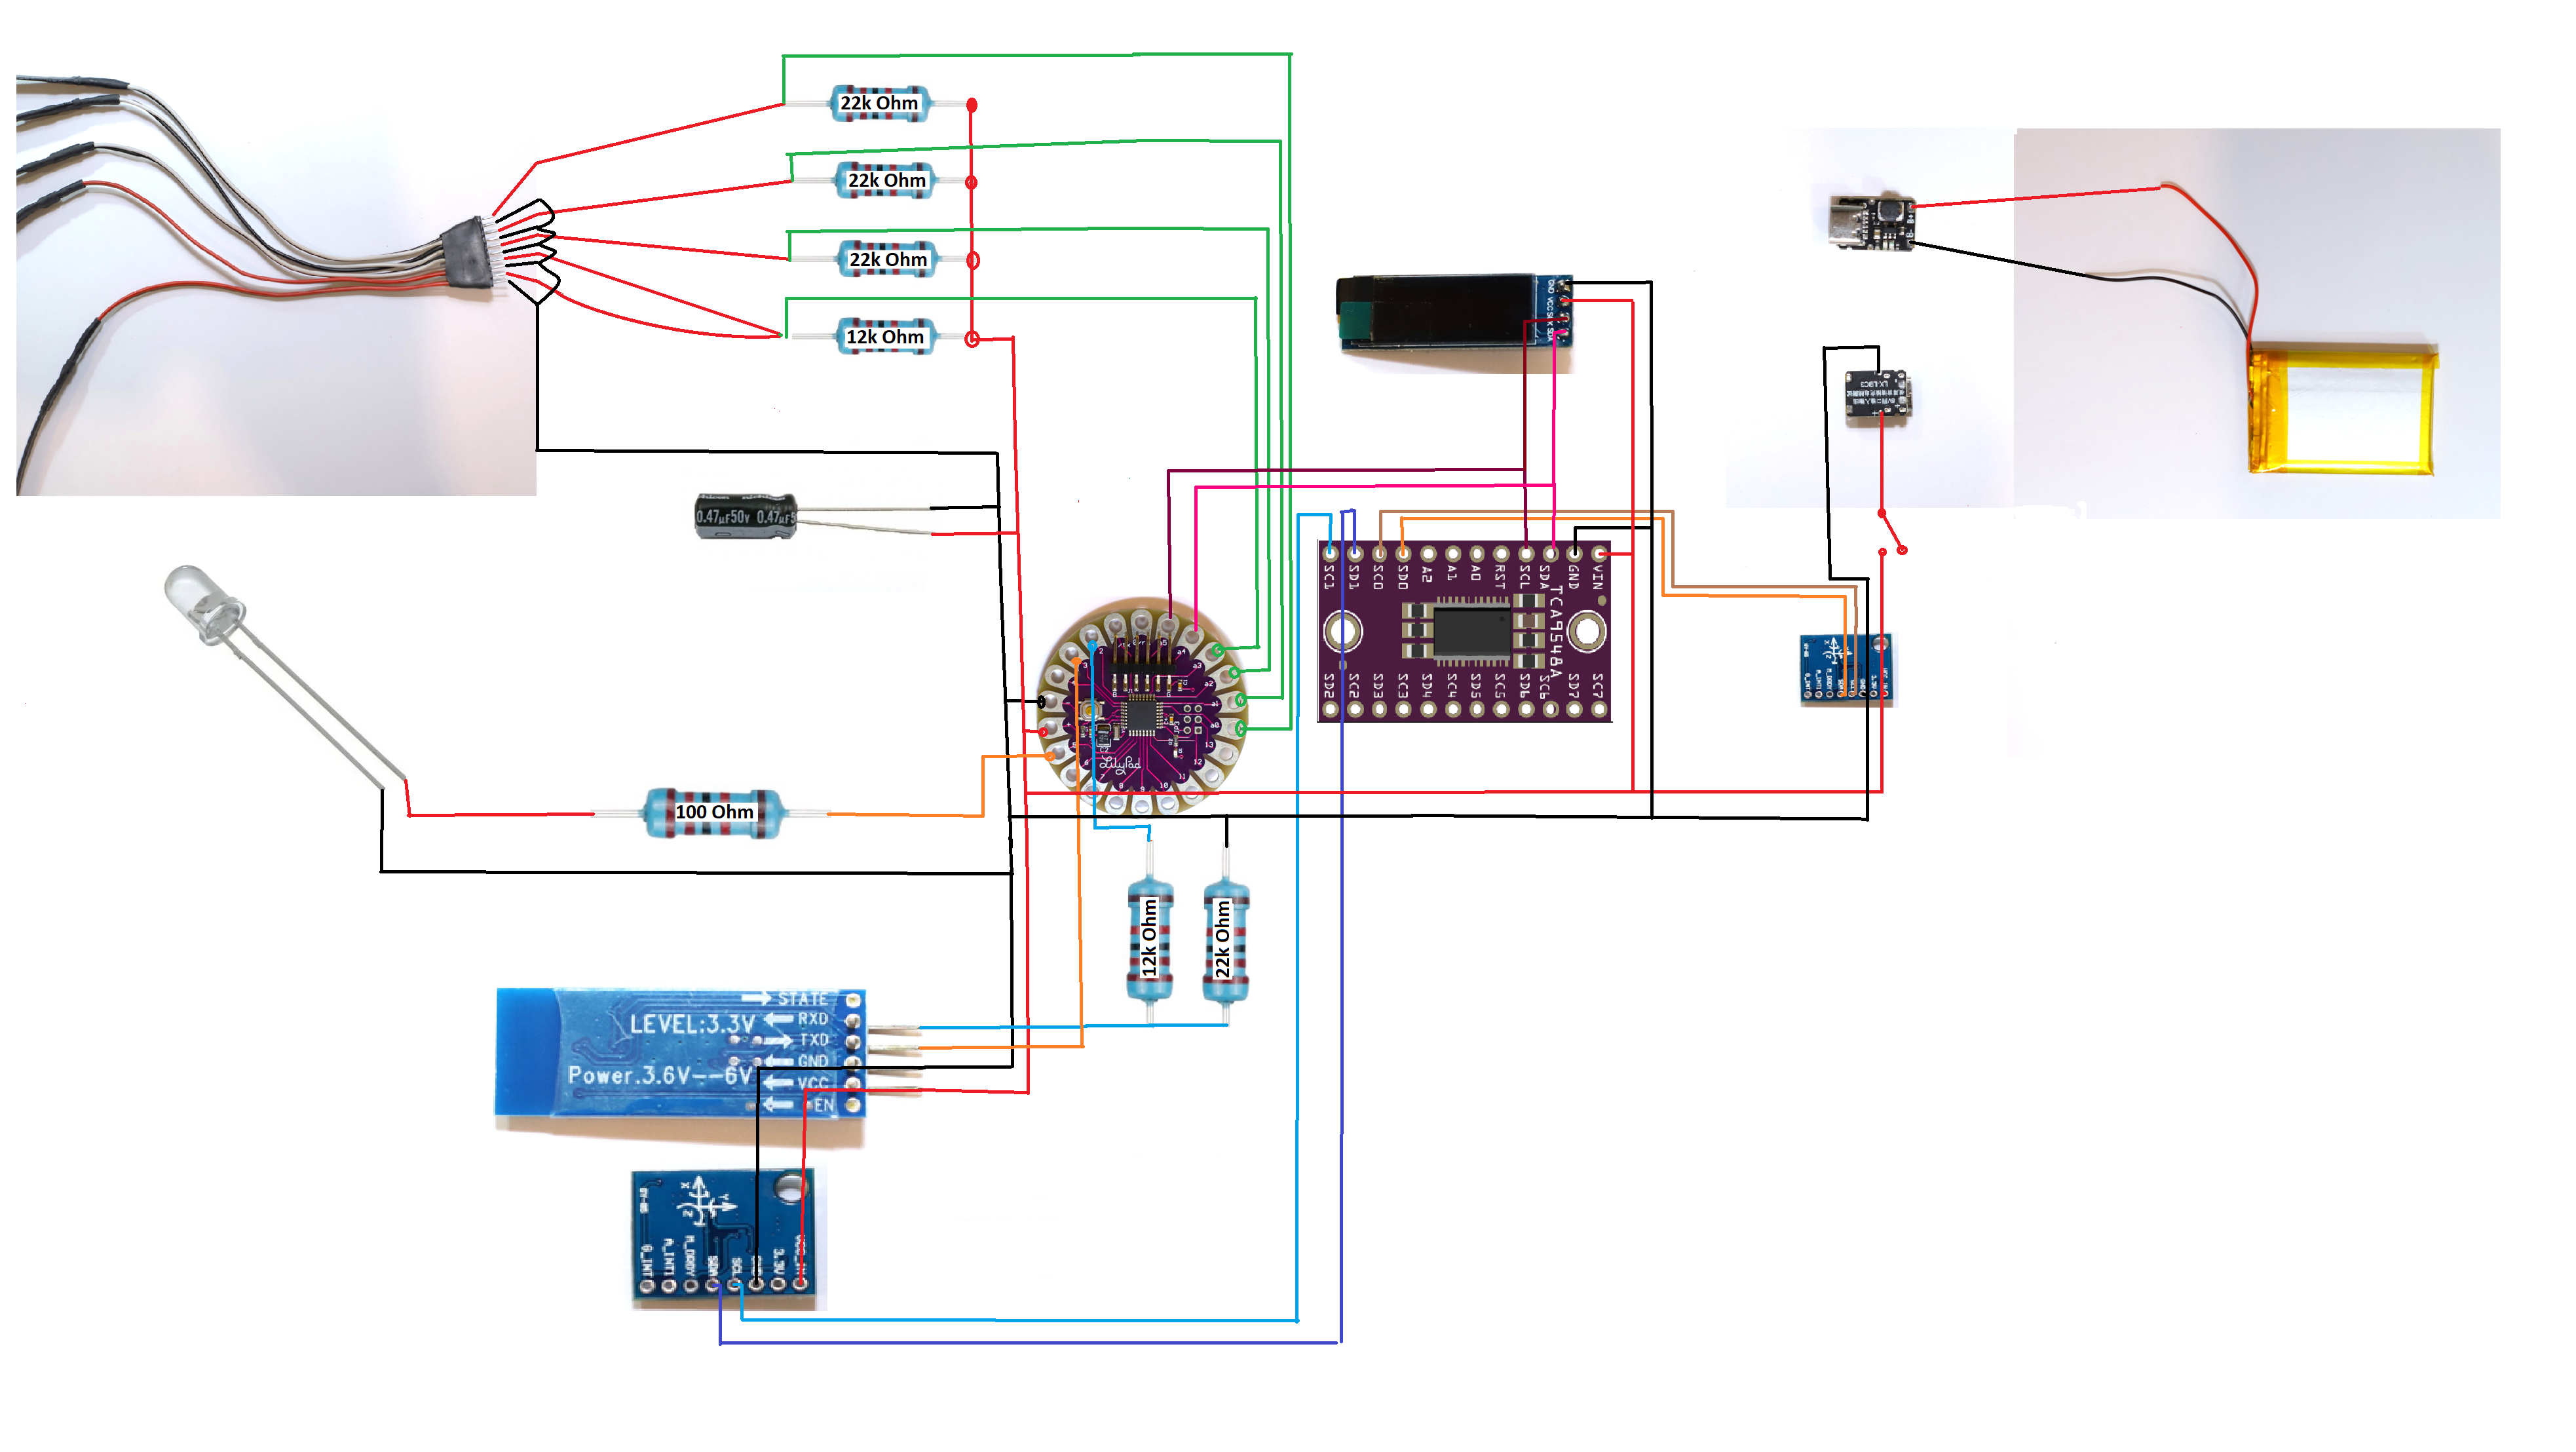
\includegraphics[width=\textwidth,height=\textheight,keepaspectratio]{Images/SystemImpl/schematic.png}
    \caption{Sơ đồ kết nối mạch}
    \label{fig:enter-label}
\end{figure}
Sơ đồ này mô tả kết nối của một mạch điện tử bao gồm nhiều thành phần như cảm biến, Arduino, màn hình hiển thị, mô-đun Bluetooth, và nguồn pin. Dưới đây là mô tả chi tiết các thành phần và kết nối của chúng:
\begin{itemize}
    \item Cảm biến Flex:\\
   - Cảm biến này có nhiều dây kết nối với các điện trở (22k Ohm và 12k Ohm).\\
   - Các dây này sau đó được kết nối với vi điều khiển (Arduino LilyPad).
   \item LED và Điện trở (100 Ohm):\\
   - LED được kết nối với một điện trở 100 Ohm và sau đó nối với vi điều khiển.
   \item Arduino LilyPad:\\
   - Đây là vi điều khiển trung tâm trong mạch, chịu trách nhiệm thu thập và xử lý dữ liệu từ các cảm biến.\\
   - Nó được kết nối với các cảm biến Flex, màn hình hiển thị, mô-đun Bluetooth và các điện trở khác.
  \item Màn hình hiển thị:\\
   - Màn hình hiển thị nhỏ (có thể là OLED) được kết nối với Arduino để hiển thị dữ liệu hoặc thông tin cần thiết.
  \item Mô-đun Bluetooth:\\
   - Mô-đun Bluetooth được kết nối để truyền dữ liệu không dây. Nó được cấp nguồn từ Arduino và được kết nối với các chân TX, RX của vi điều khiển.
  \item  Nguồn pin:\\
   - Một pin Lithium-Polymer (LiPo) được sử dụng để cung cấp năng lượng cho toàn bộ mạch.
  \item Các điện trở khác:\\
   - Có các điện trở khác trong mạch để điều chỉnh dòng điện và điện áp đi qua các thành phần.
  \item Mạch sạc và quản lý pin:\\
   - Một mạch quản lý pin (TP4056) được kết nối với pin để đảm bảo việc sạc an toàn và hiệu quả.
\end{itemize}

Dưới đây là mô tả kết nối chi tiết:

- Các dây từ cảm biến Flex được kết nối với các chân trên Arduino LilyPad thông qua các điện trở 22k Ohm và 12k Ohm.
- LED được kết nối với một điện trở 100 Ohm trước khi nối với Arduino LilyPad.
- Màn hình hiển thị được kết nối với các chân của Arduino LilyPad để hiển thị dữ liệu.
- Mô-đun Bluetooth được kết nối với các chân TX, RX, VCC, và GND của Arduino LilyPad.
- Pin LiPo cung cấp năng lượng qua mạch sạc TP4056, từ đó kết nối với Arduino và các thành phần khác để cấp nguồn.

Sơ đồ này minh họa rõ ràng cách các thành phần điện tử được kết nối với nhau để tạo thành một hệ thống hoàn chỉnh.
\begin{figure}[H]
    \centering
    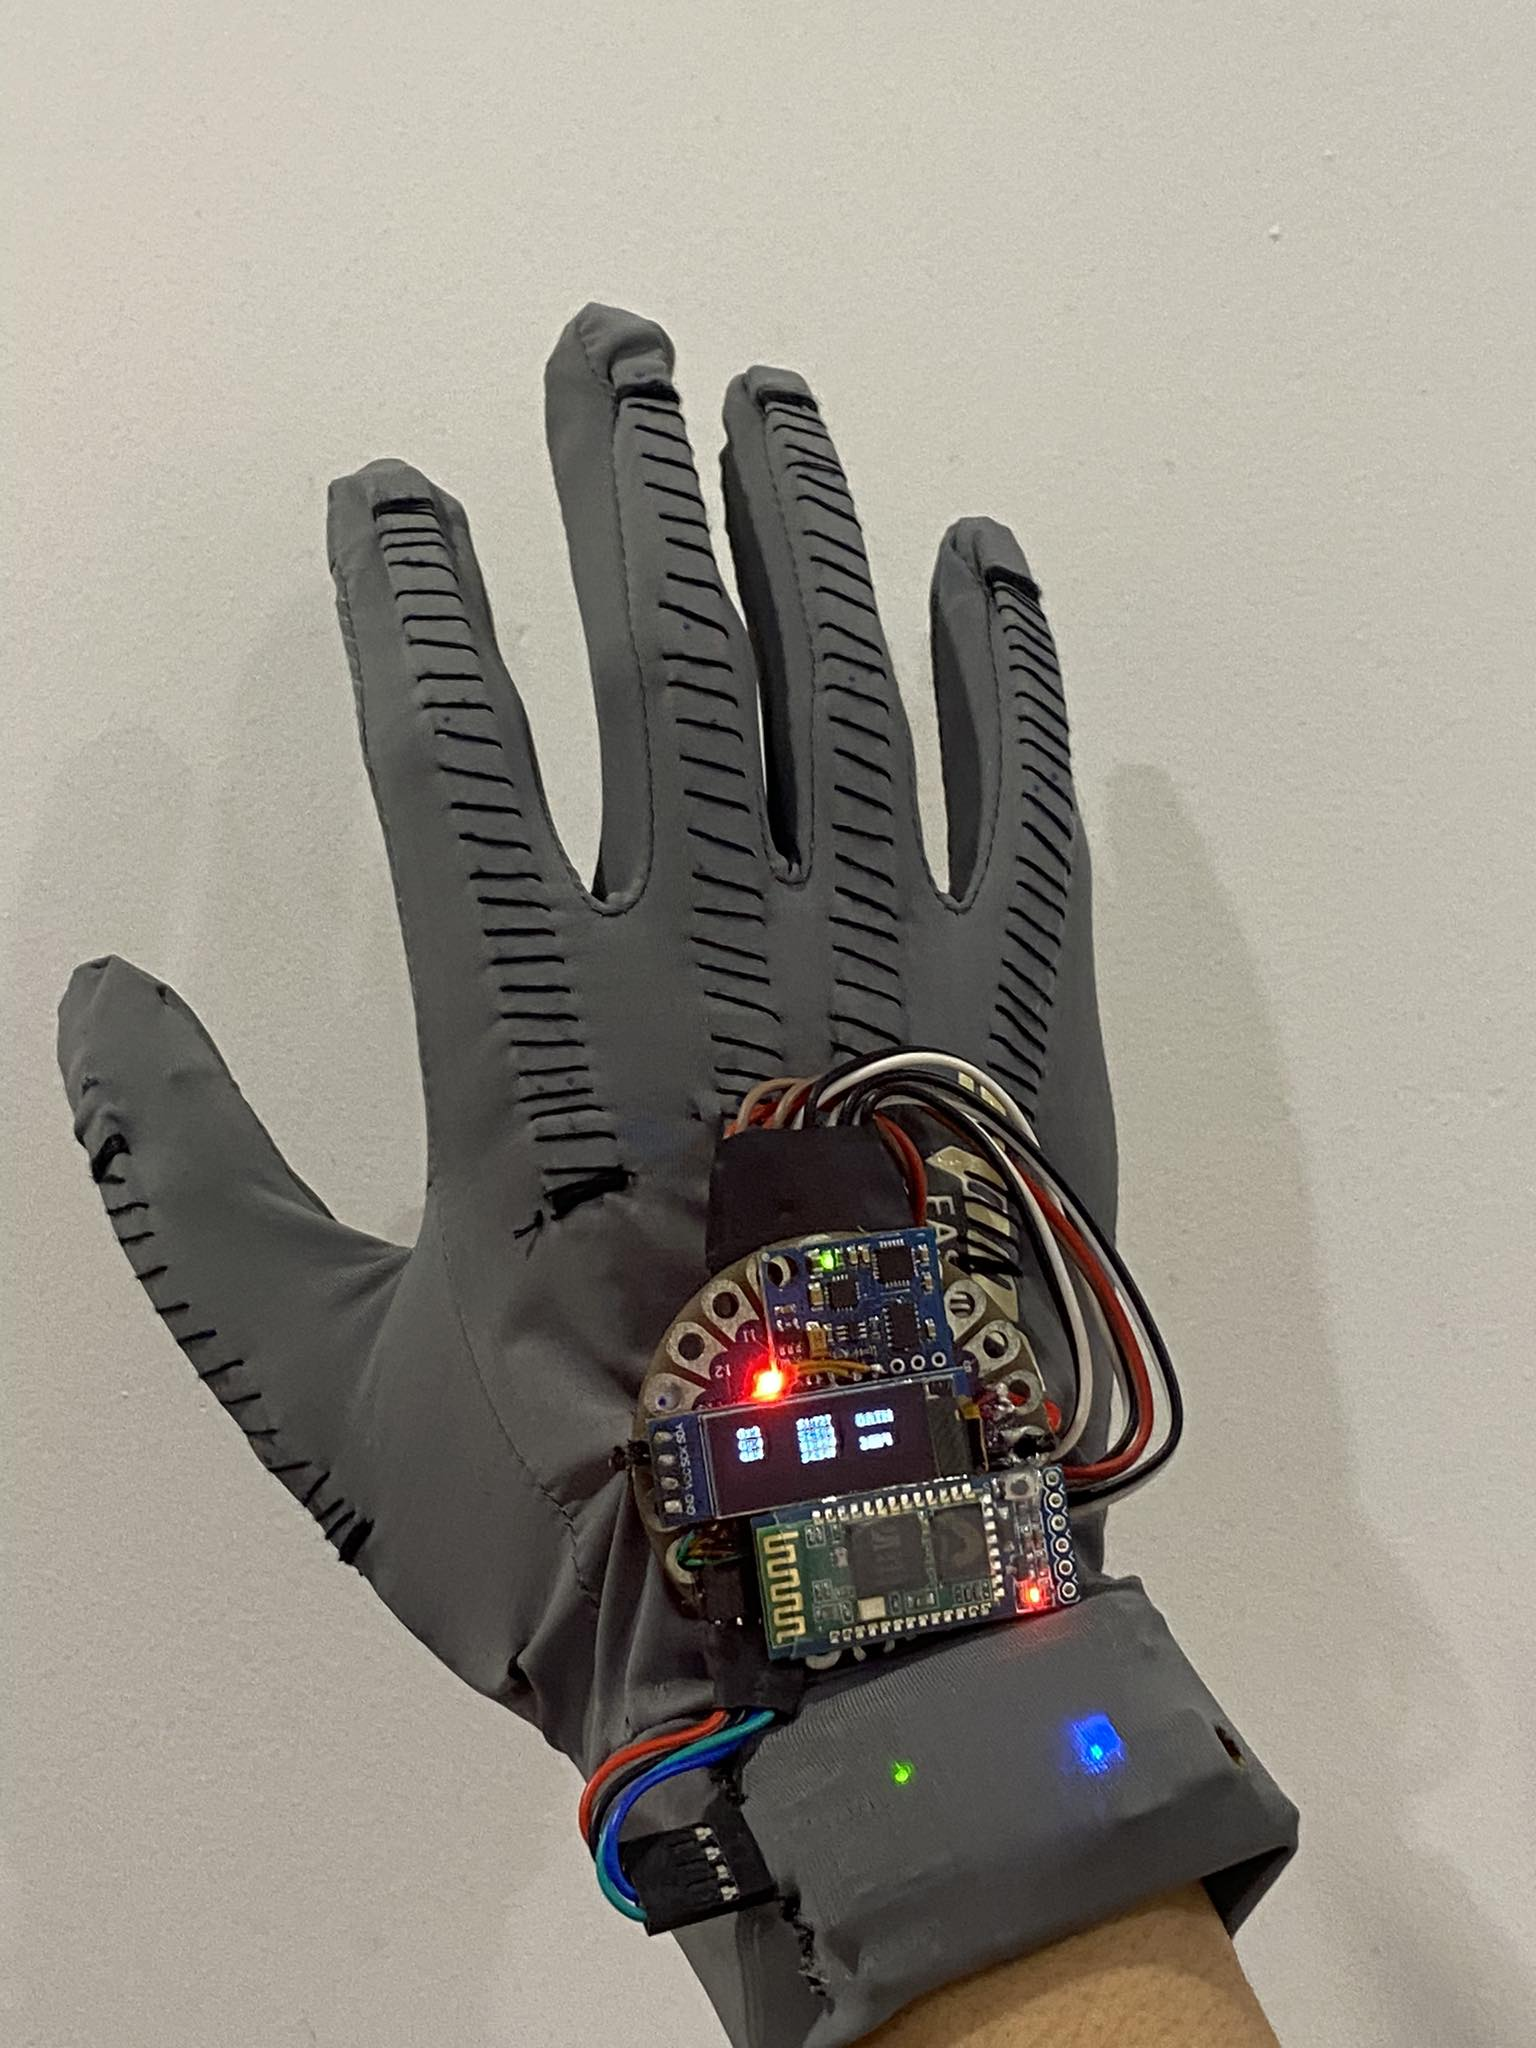
\includegraphics[width=\textwidth,height=\textheight,keepaspectratio]{Images/SystemImpl/full.jpg}
    \caption{Hình ảnh sau khi hoàn thiện}
    \label{fig:enter-label}
\end{figure}
\subsection{Xây dựng bộ dữ liệu}
Dữ liệu được thu thập từ module thu thập dữ liệu cử chỉ sau đó được lưu vào file text
\subsubsection{Dữ liệu được thu thập trên arduino}

Dữ liêu được gửi từ Arduino có 7 thành phần chính: 

\begin{lstlisting}
    gyro.readGyro(&ix,&iy,&iz); 
    ix = filter_gX.updateEstimate(ix);
    iy = filter_gY.updateEstimate(iy);
    iz = filter_gZ.updateEstimate(iz);
        readFlexSensor(flexSensor);
    flexSensor[0] = filter_flex0.updateEstimate(flexSensor[0]);
    flexSensor[1] = filter_flex1.updateEstimate(flexSensor[1]);
    flexSensor[2] = filter_flex2.updateEstimate(flexSensor[2]);
    flexSensor[3] = filter_flex3.updateEstimate(flexSensor[3]);
\end{lstlisting}

Các dữ liệu được gửi lần lượt là gia tốc trục x, gia tốc trục y, gia tốc trục z, và các tín hiệu analog 1,2,3,4. với flex 1,2 ( ngón trỏ và ngón cái) được nối song song với nhau sau đó nối tiếp đến A0, và các ngón còn lại được nối tuần tự

Đầu ra của tín hiệu được gửi qua blutetooth có dạng như sau: 
\begin{lstlisting}
"%lld\t%lld\t%lld\t%d\t%d\t%d\t%d\n"
\end{lstlisting}
 
dữ liệu được gửi với mỗi 10ms một lần

\begin{figure}[H]
    \centering
    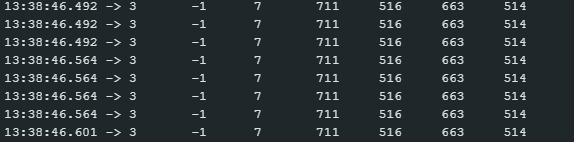
\includegraphics[width=\textwidth,height=\textheight,keepaspectratio]{Images/SystemImpl/data.png}
    \caption{Dạng dữ liêu được gửi}
    \label{fig:enter-label}
\end{figure}

\subsubsection{Dữ liệu nhận được từ gateway}
\begin{lstlisting}
SERIAL_PORT = 'COM5'
SERIAL_RATE = 38400
label = 14
DATA_FILE_NAME = './datatrain1/trainx_'+str(label)+'.txt'  # Specify the output file name
LABEL_FILE_NAME = './datatrain1/trainy_'+str(label)+'.txt'  # Specify the output file name
DATA_TEST_FILE_NAME = './datatrain1/testx_'+str(label)+'.txt'  # Specify the output file name
LABEL_TEST_FILE_NAME = './datatrain1/testy_'+str(label)+'.txt'  # Specify the output file name
test_counter = 300
queue_size = 240
windowSlide = 60
training_times = 200
testing_times = 40
\end{lstlisting}
\begin{itemize}

\item\textbf{SERIAL\_PORT} là cổng kết nối với thiết bị
Sau khi kết nối với bluetooth với arduino, kiểm tra cổng COM đã kết nối bằng cách mở phần mềm arduino

\begin{figure}[H]
    \centering
    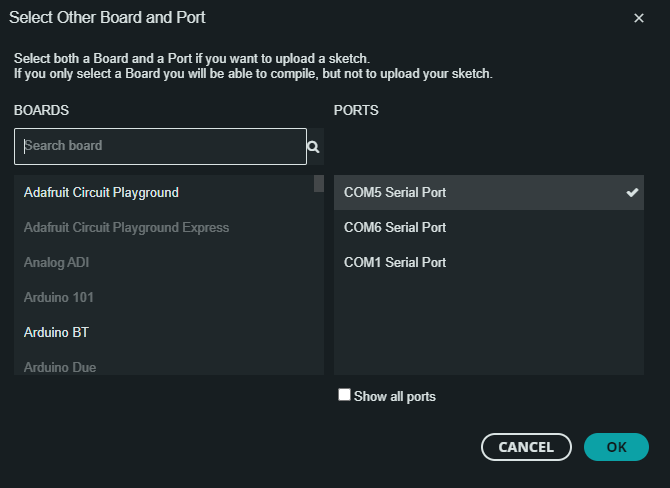
\includegraphics[width=\textwidth,height=\textheight,keepaspectratio]{Images/SystemImpl/checkcomport.png}
    \caption{kiểm tra các cổng com đang mở}
    \label{fig:enter-label}
\end{figure}

Ví dụ trong bài luận văn này là cổng 5 \\

\item\textbf{SERIAL\_RATE} ở đây là baudraute khi khởi tạo ở arduino, ở đây module bluetooth HC-05 sử dụng 38400 để đảm bảo thời gian trễ thấp nhất khi một frame dữ liệu được gửi qua\\

\item\textbf{label} là nhãn của dữ liệu khi được train,nhãn này được định nghĩa ở file config và readme như sau \\

\begin{longtblr}[
  caption = {File readme mô tả hành động được thu nhập và gắn nhãn},
]{
  width = \linewidth,
  colspec = {Q[404]Q[521]},
  hlines,
  vlines,
}
label 0          & hành động nắm tay  \\
label 1      & hành động tạm biệt ( hành động chậm)\\
label 2& hành động tạm biệt ( hành động chậm)\\                              
label 3 &chỉ vào bản thân (ngón cái đưa lên)\\
label 4 &không biết ( bàn tay xòe thẳng và xoay quanh trục ngón giữa)\\
label 5 &trạng thái nghỉ\\
label 6 &chỉ ra ngoài ( chỉ một ngón trỏ đưa lên) \\
label 7 &hành động đi bộ ( ngón giữa và ngón trỏ)\\
label 8 &ngón trỏ chỉ xuống đất và xoay vòng \\
label 9 &đùa giỡn ( ngón trỏ và ngón giữa co giãn cùng một lúc) \\
label 10 &chỉ tại đây (ngón cái và ngón giữa chỉ xuống, ngón cái đưa lên )\\
label 11 &hành động xin chào ( hành động nhanh ) \\
label 12 &giới thiệu tên \\
label 13 &thể hiện trạng thái vui vẻ ( bàn tay xòe thẳng và xoay vòng quanh cổ tay ) \\
label 14 &hành động gặp nhau ( ngón trỏ chỉ lên, các ngón còn lại co )\\
\end{longtblr}

\begin{longtblr}[
  caption = {File config là các đoạn text được chuyển sang giọng nói},
]{
  width = \linewidth,
  colspec = {Q[404]Q[521]},
  hlines,
  vlines,
}
Giữ & ~0\\
Tạm Biệt& ~1\\
Tốt lắm&~2\\
Tôi&~3\\
Không biết&~4\\
-&~5\\
Bạn&~6\\
Đi bộ&~7\\
Xung quanh&~8\\
Đùa thôi&~9\\
Tại đây&~10\\
Xin chào&~11\\
Tên là Chánh (điều chỉnh để phát ra tên như mong muốn)&~12\\
Rất vui&~13\\
Gặp&~14
\end{longtblr}

\item\textbf{DATA\_FILE\_NAME}: nơi lưu trainx\\
\item\textbf{LABEL\_FILE\_NAME}: nơi lưu trainy\\
\item\textbf{DATA\_TEST\_FILE\_NAME}: nơi lưu testx\\
\item\textbf{LABEL\_TEST\_FILE\_NAME}: nơi lưu testy\\
\item\textbf{test\_counter}: số lần test dữ liệu, được định tính trước khi bắt đầu thu thập \\
\item\textbf{queue\_size}: một frame dữ liệu để gắn nhãn cho frame đó\\
\item\textbf{windowSlide}: cửa số trượt, một lượng dữ liệu một để thêm vào một frame, trùng lặp với frame trước đó được tính bằng $queue\_size - windowSlide$
\item\textbf{training\_times}: số frame dữ liệu được ghi vào file train
\item\textbf{testing\_times}: số frame dữ liệu được ghi vào file test
\end{itemize}

Tiến hành thu thập dữ liệu với các động tác tay được định nghĩa như ở file readme
\begin{figure}[H]
    \centering
    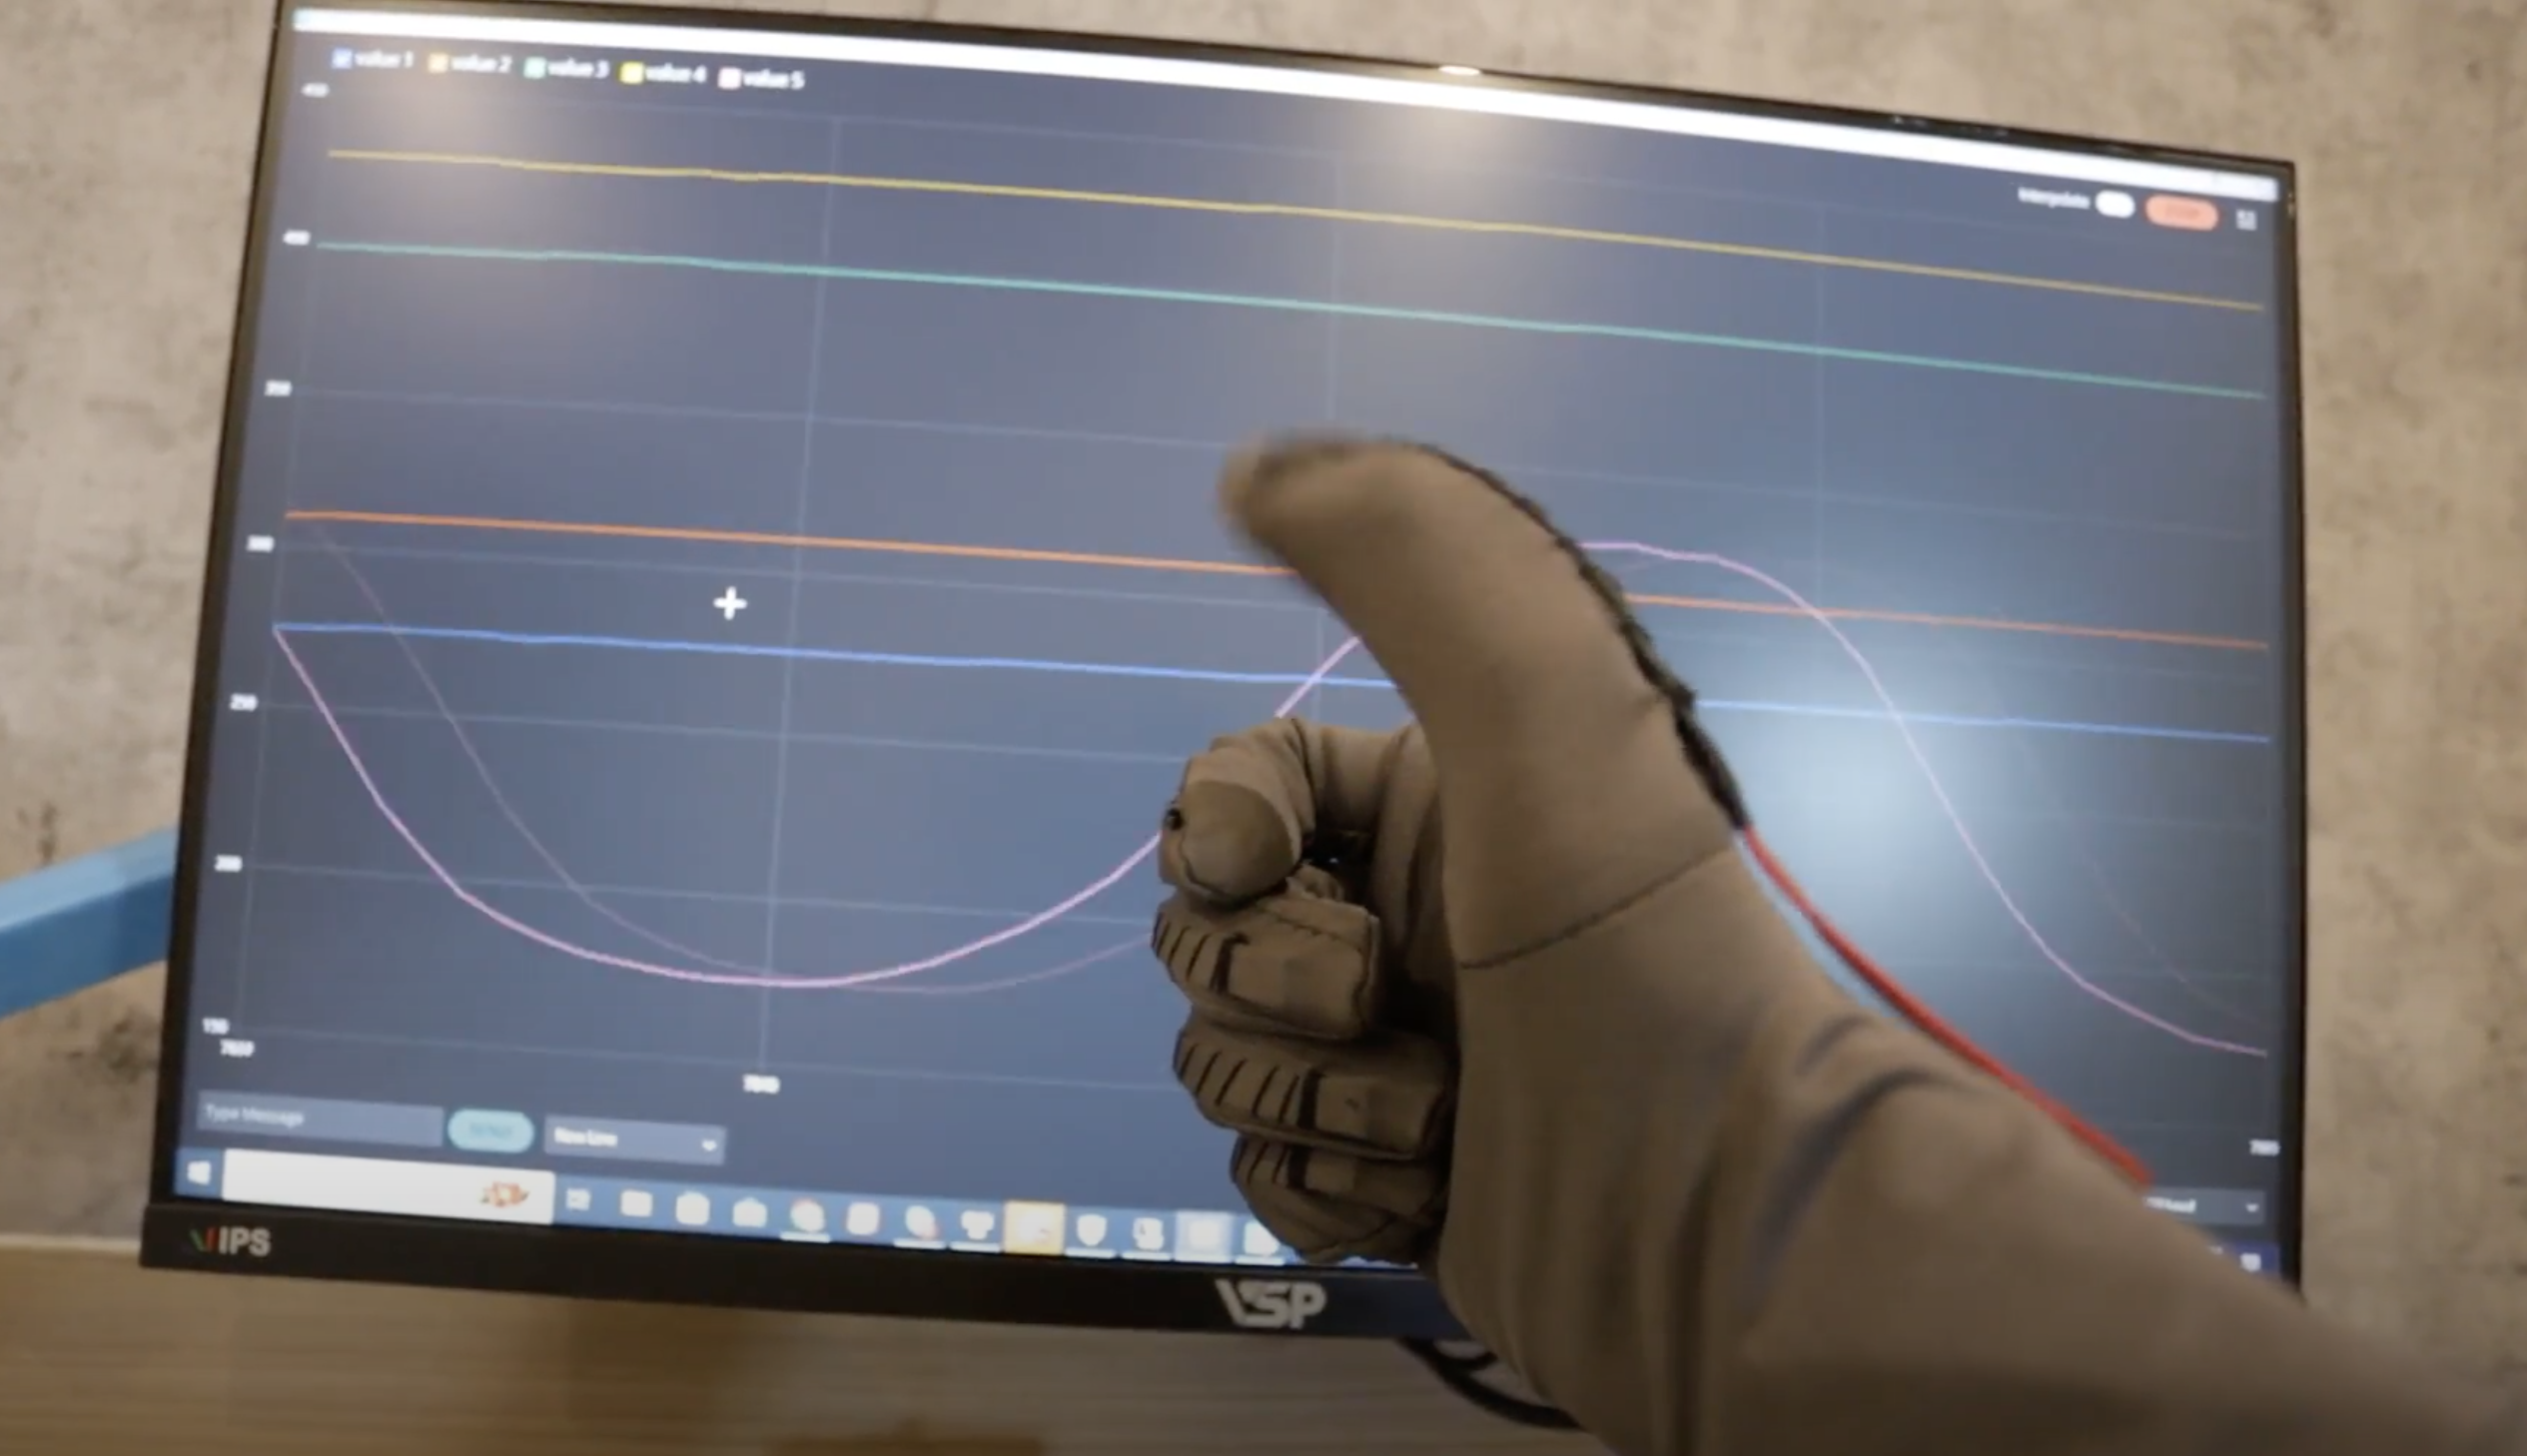
\includegraphics[width=10cm]{Images/SystemImpl/readdt_result_1.png}
    \centering
    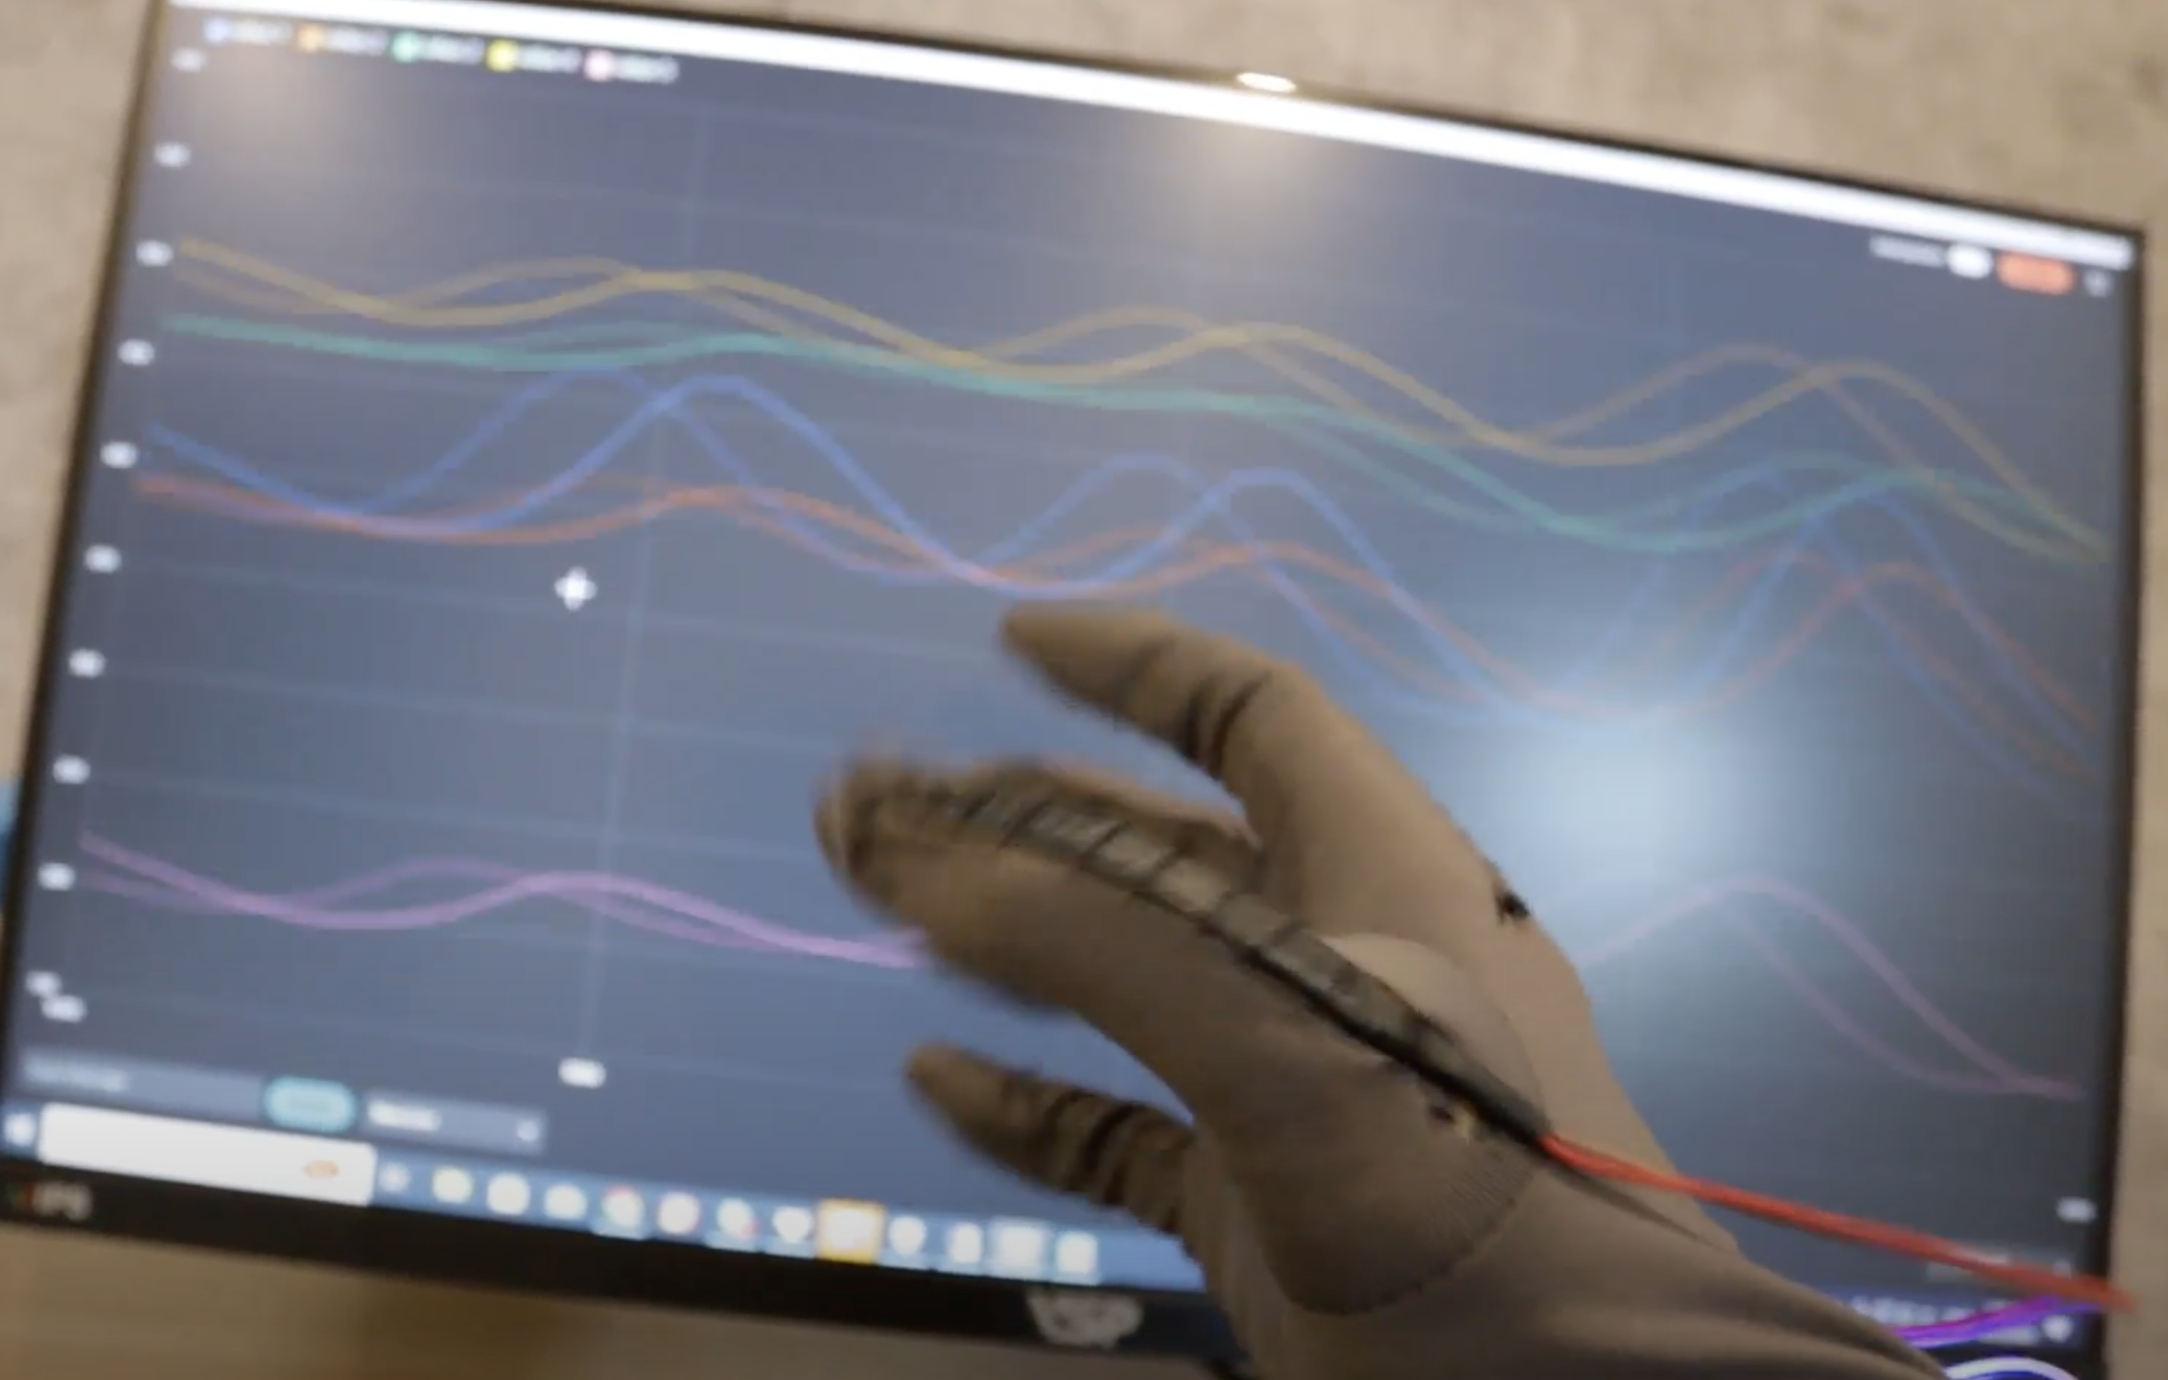
\includegraphics[width=10cm]{Images/SystemImpl/readdt_result_2.png}
\caption{Quá trình lấy dữ liệu}
\end{figure}

Các file data được lưu có kích thước cho một hành động như sau 
\begin{itemize}
    \item Một hàng có 240*7 cột dữ liệu
    \item Có tổng cộng 200 hàng dữ liệu cho file train và 20 cho trainy 
\end{itemize}
\newpage
\subsection{Định dạng data trước khi đưa vào học máy}
\begin{lstlisting}
line = next(testx).strip().split()
                if len(line) >= 1680:
                    for i in range(240):
                        x1.append(int(line[i]))
                        x2.append(int(line[i + 240]))
                        x3.append(int(line[i + 480]))
                        x4.append(int(line[i + 720]))
                        x5.append(int(line[i + 960]))
                        x6.append(int(line[i + 1200]))
                        x7.append(int(line[i + 1440]))
                else:
                    print("Error test data.")
                x1 = array(x1)
                x2 = array(x2)
                x3 = array(x3)
                x4 = array(x4)
                x5 = array(x5)
                x6 = array(x6)
                x7 = array(x7)
                line_dataset = dstack([x1, x2, x3, x4, x5, x6, x7]) 
                line_dataset = line_dataset.reshape(1,240,7)
                testx_data.append(line_dataset)
\end{lstlisting}

Có hai loại tín hiệu chính trong dữ liệu gốc: gia tốc và flexsensor
Gia tốc có 3 trục dữ liệu, flexsensor có 4 trục dữ liệu
mỗi loạt dữ liệu được ghi với thời gian là 2.4 giây
tương đương với 240 bước thời gian. Các cửa sổ dữ liệu này tương ứng với các cửa sổ đặc trưng đã được tạo ra trước đó. Điều này có nghĩa là một hàng dữ liệu có (240 * 7), tức là 1680 phần tử.

Dữ liệu sau khi được tải từ file text, sau đó được phân chia thành từng frame dữ liệu:\\
Mỗi frame dữ liệu có các tính chất như sau:
\begin{itemize}
\item Mỗi cột dữ liệu được ghi 240 lần 
\item Có tổng cộng 7 cột dữ liệu tương ứng với 7 feature của một frame

\end{itemize}
Có thể thấy hàm reshape sẽ đảm nhận việc đó
\newpage
\subsection{Xây dựng mô hình}




Sau khi train thành công dựa trên bộ dữ liệu, các tham số của mô hình được lưu vào file h5. file này được sử dụng để dự đoán các hành động










